\documentclass{article}
% !TeX spellcheck = it_IT
\usepackage{titling}
\usepackage{caption}
\usepackage{multirow}
\usepackage[T1]{fontenc}
\usepackage[utf8]{inputenc}
\usepackage[italian]{babel}
\usepackage{tabularx}
\usepackage [colorlinks=true,urlcolor=blue, linkcolor=black]{hyperref}
\newcommand{\subtitle}[1]{%
  \posttitle{%
    \par\end{center}
    \begin{center}\LARGE#1\end{center}
    \vskip0.5em}%
}

\setlength{\oddsidemargin}{0in}
\setlength{\evensidemargin}{0in}
\setlength{\topmargin}{0in}
\setlength{\headsep}{-.25in}
\setlength{\textwidth}{6.5in}
\setlength{\textheight}{8.5in}

\font\myfont=cmr12 at 40pt



\title{\myfont Norme di Progetto}
\font\myfont=cmr12 at 40pt
\date{\myfont 04-12-2018}
\begin{document}

  \maketitle
  \begin{center}
  \huge Versione 1.00 
  \\G\&B
  \end{center}
  \newpage
  \tableofcontents
  \newpage

\section*{Informazioni sul documento}


\section{Introduzione}
    \subsection{Scopo del documento}
    Questo documento si prefigge lo scopo di garantire a tutti i membri del gruppo un modo comune di lavorare al fine di aumentare l'efficenza\pedice. Verranno descritte le scelte architetturali e i vari software scelti.
    \subsection{Il prodotto}
    Il prodotto ha lo scopo di fornire un sistema "smart" di monitoraggio dei sistemi in modo da garantire e migliorare i servizi erogati dall'azienda ai terzi. L'applicativo sarà un estensione scritta in Javascript per il software Grafana, verranno inoltre utilizzate le reti bayesiane.
    \subsection{Glossario}
    Data la presenza di diversi elementi con significato ambiguo è stato necessario l'utilizzo di un glossario volto a disambiguare tali elementi col loro preciso significato.
    \subsection{Riferimenti}
    \subsubsection{Normativi}
    \begin{itemize}
        \item Standard ISO/IEC 12207:1995 \newline \url{https://www.math.unipd.it/~tullio/IS-1/2009/Approfondimenti/ISO_12207-1995.pdf}
        \item Capitolato C3 \newline \url{https://www.math.unipd.it/~tullio/IS-1/2018/Progetto/C3.pdf}
    \end{itemize}
    \subsubsection{Informativi}
    \begin{itemize}
        \item Piano di Progetto v. 1.0
        \item Piano di Qualifica v. 1.0
        \item GitHub
        \item Javascript
    \end{itemize}


\newpage

\section{Processi primari}
    \subsection{Accordo di fornitura}
    In questo paragrafo vengono documentate le norme che i membri devono seguire affinché il gruppo possa diventare committente dei professori Tullio e Cardin e diventare fornitori dell'azienda Zucchetti.
        \subsubsection{Studio di fattibilità}
        Dopo la presentazione dei capitolati il gruppo si è riunito per discutere qual'era la più consona. Dopo aver risolto i dubbi interni si è optato per la scelta del capitolato \textit{numero 3} ed infine parte del gruppo ha steso lo studio di fattibilità, documento, \textit{in versione 1.0.0},  atto a valutare i pro e i contro di ogni progetto permettendo così una più attenta valutazione. \newline
        I punti chiave dell'analisi sono i seguenti:
    \begin{itemize}
	   \item \textbf{Introduzione:} Viene fatta una breve introduzione del contesto in cui applicare la soluzione;
	   \item \textbf{Finalità: } Viene descritto in modo sintetico lo scopo finale da raggiungere a lavoro completato;
	   \item \textbf{Tecnologie in uso:} Si descrivono genericamente i software che la proponente intende usare;
	   \item \textbf{Conclusioni:} Rappresenta il motivo per cui un capitolato è stato scelto oppure scartato.
    \end{itemize}
    \subsubsection{Documentazione fornita}
    Al fine di assicurare massima trasparenza e qualità alla proponente ed ai committenti verrano elencati i documenti forniti con una breve descrizione del loro contenuto:
    \begin{itemize}
        \item \textbf{Piano di progetto:} descrive la pianificazione, la consegna e il suo completamento;
        \item \textbf{Analisi dei requisiti:} viene definita l'analisi dei casi d'uso e dei requisiti del gruppo
        \item \textbf{Piano di qualifica:} verifica e validazione e garanzia della qualità dei processi e di prodotto.
    \end{itemize}
    \subsection{Sviluppo}
    \subsubsection{Analisi dei requisiti}
    L'Analisi dei Requisiti viene scritta dagli Analisti che hanno il compito di valutare in modo accurato ogni aspetto del progetto. In particolare questo documento è redatto con lo scopo di:
    \begin{itemize}
    	\item Descrivere scopo e funzionalita' del prodotto;
    	\item Fornire i requisiti e vincoli concordati col cliente;
    	\item Descrivere gli elementi princpali che hanno un ruolo chiave nello sviluppo del prodotto;
    	\item Definire tutti i casi d'uso;
    	\item Tracciare in modo dettagliato tutti i requisiti.\newline
    \end{itemize}
    L'Analisi dei Requisiti seguira' le specifiche descritte in seguito.\newline \newline
    \textbf{Classificazione casi d'uso} Sono elencati in ordine dal più generico al più dettagliato ed è stato scelto il seguente criterio per la loro classificazione: \newline
    \begin{center}
    	UCX.Y
    \end{center}
    \begin{itemize}
    	\item \textbf{Codice X:} E' il codice identificativo del caso d'uso generico che potrebbe suddividersi
    	in casi d'uso più specifici. Nel caso non ci siano questi ultimi, il codice risulta univoco.
    	\item \textbf{Codice Y:} E' un codice identificativo univoco per il caso d'uso. E' presente solo nel
    	caso in cui il caso d'uso UCX abbia dei sotto casi d'uso più specifici.
    \end{itemize}
    X e Y sono numeri progressivi che stanno a indicare la specificità all'interno dei casi d'uso.\newline
    Ogni caso d'uso è inoltre definito secondo la seguente struttura:\newline
    \begin{itemize}
    	\item \textbf{ID:} il codice del caso d'uso secondo la convenzione specificata poco sopra;
    	\item \textbf{Nome:} titolo del caso d'uso;
    	\item \textbf{Descrizione:} breve descrizione del caso d'uso;
    	\item \textbf{Precondizione:} condizioni assunte come vere prima del verificarsi degli eventi del caso d'uso;
    	\item \textbf{Postcondizione:} condizioni assunte come vere dopo il verificarsi degli eventi del caso d'uso;
    	\item \textbf{Attori:} attori principali e secondari (se presenti) del caso d'uso;
    	\item \textbf{Scenario Principale:} flusso degli eventi rappresentato attraverso una lista numerata.\newline
    \end{itemize}
    Nell'immagine in seguito viene riportato un esempio di caso d'uso:\newline \newline
    
    \begin{figure}[hbt!]
    	\centering
    	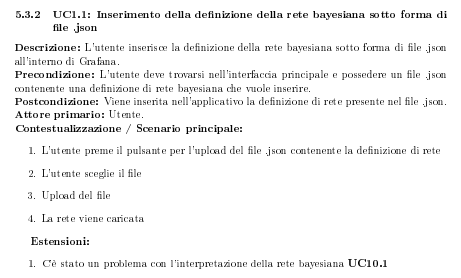
\includegraphics{casoduso.png}
    	\caption{Esempio di caso d'uso}
    \end{figure}
    
    \textbf{Classificazione dei requisiti} Tutti i requisiti ottenuti dopo una profonda analisi degli Analisti possono essere ricavati da tre diverse fonti:\newline
    \begin{itemize}
    	\item \textbf{Interno:} il requisito proviene da una decisione del gruppo DreamCorp, generalmente emersa durante un incontro e riportata in un verbale;
    	\item \textbf{Capitolato:} il requisito proviene dalle richieste del capitolato;
    	\item \textbf{Esterno:} il requisito proviene da un incontro con la proponente.\newline
    \end{itemize}
    Il codice utilizzato per indicizzare univocamente i requisiti è il seguente:\newline
    \begin{center}
    	\textbf{R+(F|Q|V|P)+(C|O)+(X(.Y)*)}
    \end{center}
    \begin{itemize}
    	\item \textbf{R:} Requisito;
    	\item \textbf{F|Q|V|P:}
    	\begin{itemize}
    		\item F: Requisito funzionale che descrive nel dettaglio i servizi che verranno forniti dal sistema agli attori;
    		\item Q: Requisito di qualità;
    		\item V: Requisito di vincolo;
    		\item P: Requisito prestazionale;
    	\end{itemize}
    	\item \textbf{C|O:}
    	\begin{itemize}
    		\item C: Compulsory (obbligatorio);
    		\item O: Optional (opzionale);
    	\end{itemize}
    	\item \textbf{X.Y:} Numeri naturali concatenati con un punto per descrivere un sottorequisito.\newline
    \end{itemize}
    I requisiti di vincolo, di qualità e prestazionali fanno parte dei requisiti non funzionali che descrivono i vincoli sul sistema e sul suo processo di sviluppo.
    Ad ogni requisito verranno infine associate la sua priorità, una breve descrizione e le sua fonti come nell'immagine in seguito.\newline
    
    \begin{figure}[hbt!]
    	\centering
    	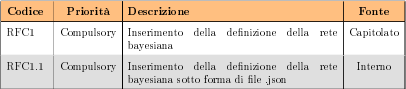
\includegraphics{requisiti.png}
    	\caption{Esempio di requisito}
    \end{figure}
    
    \textbf{Tracciamento} Infine, per facilitare la lettura e la visualizzazione dei requisiti, questi verranno indicizzati in due modalità specifiche:
    \begin{itemize}
    	\item \textbf{Tracciamento Priorità-Requisito:} il focus è orientato sulla priorità;
    	\item \textbf{Tracciamento Tipologia-Requisito:}il focus è orientato sulla tipologia.\newline
    \end{itemize}
    Per una lettura immediata non sono riportate le descrizioni per le quali si rimanda alle sezioni apposite nel documento "Analisi dei Requisiti".
    Infine viene riportata una tabella riassuntiva che permette di avere un quadro generale della distribuzione dei requisiti.\newline
    \subsubsection{Progettazione}
    L'attività di Progettazione consiste nel descrivere una soluzione al problema che sia soddisfacente per tutti gli stakeholders\pedice. Ciò serve a garantire che il prodotto sviluppato soddisfi le qualità, le proprietà e i bisogni nell'attività di analisi permettendo cosi di:
    \begin{itemize}
        \item Garantire la qualità del prodotto ;
        \item Ripartire il problema originale in maniera ricorsiva facilitando cosi la codifica delle componenti;
        \item Ottimizzare.
    \end{itemize}	
    \subsubsection{Uso di diagrammi}
    Al fine di essere il più comprensibili possibile sarà necessario far uso su larga scala di diagrammi UML\pedice 2.0
\newpage
\section{Processi di Supporto}

	\subsection{Documentazione}
		\subsubsection{Descrizione}
			In questo capitolo sono presenti le norme adottate per 	redigere, verificare e approvare la documentazione 			ufficiale prodotta da DreamCorp. Tutti documenti sono 		elencati nella sezione \hyperref[3.1.5]{\textit{\underline{3.1.5}}} denominata "Lista documenti".
		\subsubsection{Divisione dei documenti}
			Per una maggiore formalità ogni documento è stato classificato in Interno o Esterno in base alle seguenti caratteristiche:
			\begin{itemize}
				\item \textbf{Interno:} ha utilità interna al team, ovvero contiene tutte le informazioni significative per componenti del gruppo in fase di sviluppo;
				\item \textbf{Esterno:} condiviso anche con i Committenti e la Proponente, espone le informazioni utili per spiegare il metodo di lavoro seguito per lo sviluppo del progetto.
			\end{itemize}
		\subsubsection{Nomenclatura}
			I documenti formali seguono uno standard preciso per la loro nomenclatura. Di seguito un esempio esplicativo: 					\newline 
			\begin{center}
				DocumentoDiEsempio.for
			\end{center}
			\begin{itemize}
				\item \textbf{DocumentoDiEsempio:} indica il nome del documento che viene scritto utilizzando la lettera maiuscola per ogni parola presente senza spazi al suo interno;
				\item \textbf{.for:} indica il formato del documento. Quest'ultimo sarà \textit{.tex} dalla fase di creazione fino alla sua approvazione e da quel momento in poi verrà creato il file \textit{.pdf} contenente la versione definitiva di quel documento.
			\end{itemize}
			\textbf{Codice per il versionamento} La versione del documento e' specificata all'interno del documento stesso in una tabella dove sono segnate in modo preciso tutte le modifiche fatte fino ad arrivare alla major release in formato PDF. Il sistema utilizzato verrà spiegato in modo più dettagliato successivamente nella sezione \hyperref[3.2.2]{\textit{\underline{3.2.2}}} di questo documento.
		\subsubsection{Ciclo di vita documentazione}
			Per ogni documento formale sono previste tre fasi obbligatorie:
			\begin{itemize}
			\item \textbf{Redazione:} questa fase dura dalla creazione del documento fino alla scrittura completa di tutti i contenuti previsti. Durante questo processo, il Responsabile di Progetto assegna ai Redattori i contenuti da aggiungere e una volta che quest'ultimi saranno esauriti potrà approvare il passaggio alla fase successiva;
			\item \textbf{Verifica:} in questa fase il documento viene controllato in ogni sua parte attraverso le opportune procedure dai Verificatori che una volta ultimato il lavoro daranno il loro feedback al Responsabile di Progetto; questo può dunque approvare il documento che passa quindi alla fase successiva oppure può farlo tornare alla fase di Redazione per correggere eventuali imperfezioni riscontrate dai Verificatori;
			\item \textbf{Approvato:} In questa fase il documento e' pronto per essere rilasciato e la sua versione viene aggiornata ad una major.
			\end{itemize}
		\subsubsection{Lista documenti}
		\label{3.1.5}
			\begin{itemize}
				\item \textbf{Analisi dei Requisiti: }[Esterno] \newline
				Il suo scopo è di analizzare ed esporre i requisiti del progetto. Contiene l'analisi dei casi d'uso che riguardano il prodotto in fase di sviluppo e i diagrammi di interazione con l'utente a prodotto ultimato;
				\item \textbf{Norme di Progetto: }[Interno] \newline
				Contiene tutte le regole e le convenzioni adottate dai membri del gruppo DreamCorp per uno sviluppo metodico del progetto;
				\item \textbf{Piano di Progetto: }[Esterno] \newline
				Il suo scopo è quello di descrivere gli obiettivi del progetto e gli elementi necessari per il loro raggiungimento. Inoltre vien presentato come il gruppo DreamCorp amministra il proprio tempo e i membri al suo interno;
				\item \textbf{Piano di Qualifica: }[Esterno] \newline
				Consiste in una spiegazione dettagliata di come il team DreamCorp vuole soddisfare i requisiti di qualità del progetto;
				\item \textbf{Studio di Fattibilità: }[Interno] \newline
				Il suo obiettivo è di mostrare come è stato analizzato ogni capitolato elencando per ognuno punti a favore e sfavore in modo da evidenziare tutti i dubbi sorti in fase di decisione.
				\item \textbf{Glossario: }[Esterno] \newline
				Contiene tutti i termini presenti nei documenti formali che il gruppo DreamCorp ha ritenuto opportuno avessero bisogno di una spiegazione o chiarimento per facilitarne la comprensione. E' unico per tutti i documenti.
			\end{itemize}
		\subsubsection{Norme tipografiche}
			Le norme scritte in questa sezione devono essere seguite in tutti i documenti prodotti dal team DreamCorp:
			\begin{itemize}
				\item \textbf{Date:} sono scritte seguendo la regola anno-mese-giorno (YYYY-MM-DD);
				\item \textbf{Voci nel Glossario:} per segnalare una parola che si trova nel glossario viene posta una \textbf{G} a pedice della parola;
				\item \textbf{Link interni:} i collegamenti che rimandano a una sezione interna al documento sono scritti in corsivo e sottolineati;
				\item \textbf{Link esterni:} i collegamenti che rimandano a una pagina web esterna al documento sono scritti in colore blu;
				\item \textbf{Elenchi puntati:} ogni elemento della lista è caratterizzato in generale da una prima parola o serie di parole in grassetto seguite da due punti \textit{":"} e successivamente dal suo contenuto, ma può anche essere formato solamente dal contenuto nei casi in cui non sia necessaria una particolare specifica iniziale. Alla fine è posto un punto e virgola \textit{";"} tranne per l'ultimo elemento che è concluso da un punto \textit{"."};
				\item \textbf{Citazioni:} le citazioni sono scritte in \textit{corsivo}.
			\end{itemize}
		\subsubsection{Struttura dei documenti}
			Tutti i documenti utilizzano una struttura di base contenuta nel file \textit{stile.tex} in modo da non ripetere ogni volta gli elementi comuni.
			\newline \newline \textbf{Frontespizio} E' la prima pagina del documento dove si trovano:
			\begin{itemize}
				\item \textbf{Logo:} immagine identificativa del gruppo;
				\item \textbf{Nome del progetto:} G\&B;
				\item \textbf{Nome del documento};
				\item \textbf{Data:} data in cui è stato approvata la versione corrente in cui è stato approvato il documento;
				\item \textbf{Versione:} versione corrente del documento;
				\item \textbf{Nome del gruppo:} DreamCorp.
			\end{itemize}
			In seguito in forma tabellare sono riportati:
			\begin{itemize}
				\item \textbf{Responsabile:} persona a capo del progetto nel momento in cui è stato approvato;
				\item \textbf{Redattori:} persone incaricate nella stesura del documento;
				\item \textbf{Verificatori:} persone incaricate di controllare la qualità del documento;
				\item \textbf{Stato:} punto del ciclo di vita nel quale si trova il documento;
				\item \textbf{Classificazione:} Interno o Esterno;
				\item \textbf{Destinatari:} persone alle quali è destinate il documento.
			\end{itemize}
		\textbf{Diario delle modifiche}  Si trova a partire dalla seconda pagina del documento e riporta sotto forma di tabella tutte le modifiche apportate al documento. La tabella è composta da quattro colonne che contengono rispettivamente descrizione della modifica, autore della modifica, data della modifica e versione a cui è arrivato il documento.
		\newline \newline \textbf{Indice}  E' posto sempre dopo il Diario delle Modifiche e contiene l'elenco dei capitoli e sottocapitoli in cui è diviso il documento.
		\newline \newline \textbf{Contenuto}  Il documento è completato dal suo contenuto. Ogni pagina è composta come di seguito:\newline
		\begin{itemize}
			\item \textbf{Logo del team:} in alto a sinistra nell'intestazione;
			\item \textbf{Capitolo:} in alto a destra nell'intestazione;
			\item \textbf{Contenuto:} occupa l'intera pagina;
			\item \textbf{Nome Documento:} in basso a sinistra nel piè di pagina;
			\item \textbf{Numero Pagina:} in basso a destra nel piè di pagina. \newline
		\end{itemize}
		L'intestazione e il piè di pagina sono separate dal resto del documento attraverso due righe nere orizzontali. Ogni nuovo capitolo (identificato in \LaTeX ~con il comando \textit{\textbackslash{}section}) comincia sempre in una nuova pagina.
		\subsubsection{Strumenti di supporto}
			Il formato scelto per la stesura della documentazione è il  \LaTeX ~che permette una maggiore precisione e uniformità fra tutti i membri del gruppo. L'ambiente di sviluppo scelto è \textbf{TeXstudio\pedice} il quale è risultato il più completo in termini di funzioni e praticità.
	\subsection{Versionamento}
		E' stata scelta la tecnologia Git per le parti del progetto e della documentazione che necessitano di un versionamento e il servizio utilizzato è GitHub. Per tutte le altre parti lo strumento di condivisione di cui si serve il gruppo DreamCorp è una cartella su Google Drive\pedice.
		\subsubsection{Comandi di base}
			In seguito vengono descritti i comandi principali di cui si è servito il team per l'uso di Git all'interno del progetto:
			\begin{itemize}
				\item \textbf{git clone:} crea una copia in locale del repository\pedice;
				\item \textbf{git pull:} aggiorna la cartella in locale col contenuto del repository in remoto;
				\item \textbf{git checkout:} permette di cambiare branch\pedice su cui si sta lavorando;
				\item \textbf{git add:} aggiunge uno o più file a seconda del comando alla lista dei file tracciati da Git. Aggiungendo il simbolo "." si possono aggiungere tutti i file modificati con un solo comando;
				\item \textbf{git commit -m "\textit{Messaggio}":} fa il commit\pedice delle modifiche effettuate in locale di tutti i file che sono stati aggiunti attraverso il comando \textit{git add}. Il messaggio da inserire non è opzionale e deve descrivere lo scopo del commit;
				\item \textbf{git push:} carica in remoto le modifiche effettuate in locale;
				\item \textbf{git status:} permette di consultare  lo stato del repository locale mostrando i file tracciati e non. \newline
			\end{itemize}
			Inoltre, per migliorare il workflow generale è stato utilizzato GitFlow che permette una gestione più accurata dei branch.
		\subsubsection{Numerazione della versione}
		\label{3.2.2}
			La versione di tutti i documenti è rappresentata nella forma X.Y.Z seguendo le seguenti regole:
			\begin{itemize}
				\item \textbf{X:} è il numero di una major release che avviene una volta che il documento passa allo stato di Approvato;
				\item \textbf{Y:} numero di una release normale nella quale sono state apportate modifiche o aggiunte sostanziali al documento;
				\item \textbf{Z:} è il numero di una minor release nella quale vengono apportate piccole modifiche o correzioni.
			\end{itemize}
		L'aumento di una cifra comporta l'azzeramento di quelle alla sua destra. \newline
	\subsection{Verifica}
		\subsubsection{Analisi statica}

		\subsubsection{Analisi dinamica}

		\subsubsection{Strumenti di verifica}
\newpage
\section{Processi organizzativi}
    \subsection{Comunicazione}
        In questa sezione vengono le presentate le norme per la comunicazione tra le parti che aderiscono al progetto.
        \subsubsection{Comunicazioni interne}
            Vengono di seguito esposte le metodologie di comunicazione all'interno del team DreamCorp.
            \newline
            Per le comunicazioni all'interno del gruppo è stato utilizzato \textit{Slack}\pedice, un'applicazione di messaggistica multipiattaforma adatto per i gruppi di lavoro. Attraverso questo strumento è possibile suddividere lo spazio di comunicazione in canali tematici, ricercare messaggi, condividere file di grosse dimensioni e tracciare i messaggi.
            \newline
            All'interno di \textit{Slack} sono stati predisposti dei canali tematici al fine di rendere più efficiente lo scambio di messaggi:
            \begin{itemize}
                \item \textbf{general}: Canale utilizzato per le comunicazioni e l'organizzazione di carattere generale;
                \item \textbf{github-notificaton}: Canale a cui è stato aggiunto un bot di GitHub il quale permette di inviare un messaggio nel momento in cui un membro del team apre/chiude issues, effettua un merge o una \textit{push};
                \item \textbf{automatismi}: Dove si discute dei software da utilizzare per creare automatismi;
                \item{random}: Canale generico dove discutere di tutto ciò che non è inerente al progetto.    
            \end{itemize}
            
            Inoltre sono stati predisposti dei canali per la redazione dei documenti, uno per ogni documento, in modo da facilitare la discussione degli stessi:
            \begin{itemize}
                \item \textbf{norme\_di\_progetto}: Utilizzato per discutere delle norme di progetto da seguire durante lo sviluppo;
                \item \textbf{piano\_progetto}: Canale riservato alla redazione del documento \textit{Piano di progetto};
                \item \textbf{studio\_di\_fattibilita}: Canale per la raccolta delle considerazioni sui capitolati e per la scrittura del documento;
                \item \textbf{piano\_di\_qualifica}: Utilizzato per discutere del raggiungimento della qualità e per l'organizzazione della redazione del documento;
                \item \textbf{analisi\_requisiti}: Per discutere dei casi d'uso, requisiti e utilizzo del software per la redazione del documento \textit{Analisi\_dei\_requisiti}; 
                \item \textbf{glossario}: Dove viene confrontato il contenuto dei glossari personali.
            \end{itemize}
            
            I membri del team sono tenuti a comunicare rispettando i topic, nel caso si volesse portare all'attenzione tutti i membri del gruppo sono presenti i comandi:
            \begin{itemize}
                \item \textit{@everyone} per notificare tutti i membri del gruppo;
                \item \textit{@channel} per notificare i membri di un specifico canale.
            \end{itemize}
            
          
            Altre modalità di comunicazione previste sono:
            \begin{itemize}
                \item Comunicazioni orali informali: per parlare di qualsiasi problematica, strategia, utilizzo di strumenti, consigli, dubbi;
                \item Riunioni: Incontri di persona precedentemente organizzati.
            \end{itemize}        
        \subsubsection{Comunicazioni esterne}
            Questa sezione è inerente alle modalità di comunicazione da seguire con i membri esterni al gruppo di lavoro.
            \newline
            Allo scopo di garantire un costante miglioramento della qualità di prodotto, sono stati individuati le seguenti entità esterne:
            \begin{itemize}
                \item La proponente \textbf{Zucchetti S.p.a}, rappresentata da Gregorio Piccoli, board member e CTO dell'azienda, con il quale si vuole stabilire un rapporto di collaborazione per definire bisogni e requisiti per la realizzazione del prodotto;
                \item I Committenti \textbf{Prof. Tullio Vardanega} e \textbf{Prof. Riccardo Cardin}, ai quali verrà consegnata tutta la documentazione in ciascuna fase di revisione, con i quali si vuole stabilire un rapporto utile al miglioramento dei processi e delle strategie.
            \end{itemize}
            \paragraph{Comunicazioni esterne scritte} Devono essere effettuate tassativamente attraverso l'uso dell'indirizzo mail del gruppo:
            \newline
            dreamcorp.swe@gmail.com   **********DA MODIFCARE***********
            \newline
            Ogni email ricevuta a questo indirizzo verrà inoltrata automaticamente alla casella postale di ogni membro del gruppo attraverso l'utilizzo dei filtri di Gmail\pedice, inoltre il testo delle mail verrà riportate come messaggio su \textit{Slack} attraverso l'uso di un bot.
            \paragraph{Composizione email}
            Viene di seguito presentata la modalità di scrittura delle email rivolte a soggetti esterni.
            \begin{itemize}
                \item \textbf{Email verso la Proponente Zucchetti S.p.a} 
                \item \textbf{Email verso i Committenti}: ci si propone di utilizzare un oggetto che descriva in modo più accurato possibile il contenute del messaggio, ai committenti ci si rivolgerà con il Voi e con il Lei.
            \end{itemize}
            Nella possibilità in cui un messaggio debba essere mandato a più persone, nel campo "A:" va indicato il principale destinatario, mentre nel campo "Cc:" vanno indicati tutti gli altri.
            Viene posta particolare attenzione nella modalità di risposta e di inoltro delle email. In questi casi sono da utilizzare i tasti "Rispondi a tutti" e "Inoltra a" che formatteranno in automatico il corpo del messaggio includendo le clausole "Re:" e "I:".
            \subsection{Riunioni}
                In questa sottosezione vengono presentate le modalità di riunione, sia interne che esterne.
                Allo scopo di far rispettare l'ordine del giorno, redigere il \textit{Verbale di riunione} e prendere nota degli argomenti trattati e delle decisioni prese, all'interno di ogni riunione dovrà essere nominato a turno tra i membri del gruppo DreamCorp un Segretario.
                \subsubsection{Verbali di riunione}
                   Nello svolgimento delle riunioni è compito del Segretario redigere il documento \textit{Verbale di riunione} secondo il seguente schema:
                    \begin{itemize}
                        \item \textbf{Verbale Esterno DATA}, incluso nel frontespizio. Per DATA si intende la data in cui è stata effettuata la riunione, scritta secondo le \textit{Norme Tipografiche};
                        \item \textbf{Informazioni sulla riunione}: sezione contente:
                        \begin{itemize}
                            \item \textbf{Motivo}: Descrizione sintetica del motivo che ha portato ad indirre una riunione;
                            \item \textbf{Luogo e Data}: ad esempio \textit{Padova, Giovedì 23 Febbraio 2019}; 
                            \item \textbf{Ora inizio}: nel formato ventiquattro ore;
                            \item \textbf{Ora fine}: nel formato ventiquattro ore;
                            \item \textbf{Partecipanti}: vengono elencati i partecipanti della riunione, iniziando dal Proponente/Committente nel caso la riunione sia esterna. Nel caso un membro sia costretto a lasciare la riunione prima del previsto, deve essere annotata l'ora di uscita e il motivo.
                        \end{itemize}
                        \item \textbf{Ordine del giorno}: Un elenco puntato degli argomenti discussi; 
                        \item \textbf{Resoconto}: sezione contente le annotazioni circa le decisioni prese con motivazioni e gli argomenti discussi e non.
                    \end{itemize}
                    \paragraph{Nomenclatura} 
                        I verbali esterni dovranno avere nome:
                        VER-DATA
                        \newline
                        I verbali interni saranno nominati:
                        VIR-DATA
                        \newline
                        Viene usata questa nomenclatura al fine di avere una facile consultazione.
                        \newline
                    \paragraph{Conservazione dei verbali}
                        I verbali interni ed esterni verranno redatti in \LaTeX e caricati nel repository del progetto.
                \subsubsection{Riunioni interne}
                    La partecipazione delle riunioni interne è permessa ai soli membri del gruppo DreamCorp.
                    \newline
                    \paragraph{Compiti del Responsabile di Progetto}
                        Di seguito vengono elencati i compiti che deve eseguire il Responsabile di Progetto:
                        \begin{itemize}
                            \item Fissare la data delle riunioni interne, previa discussione con i membri all'interno del canale \textit{general} su \textit{Slack};
                            \item Stabilire l'ordine del giorno;
                            \item Valutare le richieste di riunione dei membri del gruppo e decidere se accettarle;
                            \item Comunicare data e ordine del giorno attraverso il comando \textbf{@everyone} all'interno di \textit{Slack} con almeno un giorno di anticipo;
                            \item Verificare ed approvare il verbale;
                            \item Confermare spostare od annullare le riunioni sempre con le modalità di notifica a tutti i membri del gruppo.
                         \end{itemize}
                     \paragraph{Compiti dei partecipanti}
                        \begin{itemize}
                            \item Comunicare tempestivamente assenze e/o ritardi; 
                            \item Presentarsi puntualmente alle riunioni;
                            \item Partecipare attivamente alle discussioni;
                            \item Mantenere un atteggiamento educato.
                        \end{itemize}
                    \paragraph{Approvazione delle decisioni}
                        Le decisioni vengono approvate con la regola della maggioranza dei partecipanti alla riunione.
                        Affinché una riunione sia valida devono essere presenti almeno cinque membri del gruppo.
                        
                  \subsubsection{Riunioni esterne}
                  
            \subsection{Ruoli di progetto}
                Nonostante il progetto sia collaborativo, all'interno del gruppo sono stati assegnati dei ruoli corrispondenti alle figure aziendali, essi sono:
                \begin{itemize}
                    \item \textbf{Responsabile di progetto};
                    \item \textbf{Amministratore};
                    \item \textbf{Progettista};
                    \item \textbf{Verificatore};
                    \item \textbf{Programmatore}.
                \end{itemize}
                I ruoli verranno assegnati inizialmente verranno ruotati secondo un calendario prescritto nel documento \textit{Piano di Progetto}
                Si cercherà evitare situazioni di conflitto d'interesse, come per esempio attuare la verifica di un documento da parte del redattore dello stesso.
                \subsubsection{Responsabile di Progetto}
                    La figura di "Project Manager", o Responsabile di progetto, è responsabile unica dell'avvio, pianificazione, esecuzione, controllo e chiusura di un progetto facendo ricorso a tecniche e metodi  di project management. Egli partecipa al progetto dalla sua  fine.
                    \newline
                    I compiti principali del Project Manager sono:
                    \begin{itemize}
                        \item Elaborare la pianificazione e la programmazione di dettaglio;
                        \item Organizzare efficientemente ed efficacemente le risorse umane a sua disposizione;
                        \item Favorire la comunicazione e l'affiatamento del team di progetto;
                        \item Distribuire le risorse sulle attività e monitorarne lo svolgimento;
                        \item Prendere tutte le iniziative volte a prevenire i rischi;
                        \item Mantenere i contatti con gli utenti di riferimento e gli utenti finali pianificandone il coinvolgimento nelle varie attività del progetto;
                        \item Produrre la documentazione di sua competenza e supervisionare quella prodotta dal team di progetto;
                        \item Controllare la qualità dei prodotti parziali ed assicurarsi che gli standard di qualità adottati siano rispettati;
                        \item Avere sempre un'attenzione particolare al miglioramento dei processi produttivi del progetto.
                    \end{itemize}
                \subsubsection{Amministratore}
                    L'Amministratore è colui che controlla l'ambiente di lavoro e che si preclude l'obiettivo di aumentare la qualità del lavoro dando strumenti al gruppo di lavoro.
                    I principali compiti dell'Amministratore sono:
                    \begin{itemize}
                        \item Amministrare le infrastrutture di supporto;
                        \item Risolvere i problemi riguardo la gestione dei processi;
                        \item Assicurare che la documentazione sia corretta, verificata, approvata, aggiornata e versionata;
                        \item Controllare le versioni e configurazioni dei prodotti;
                        \item Dare regole e procedure per lo svolgimento del lavoro.
                    \end{itemize}
                \subsubsection{Progettista}
                    Il Progettista è colui che redige il Progetto, ha un proprio bagaglio culturale e una congrua esperienza. Egli:
                    \begin{itemize}
                        \item Concorre in prima persona allo sviluppo del progetto;
                        \item Supervisiona lo sviluppo software;
                        \item Controlla le attività svolte dal gruppo di lavoro;
                        \item Forma il personale e soggetti esterni.
                    \end{itemize}
                \subsubsection{Verificatore}
                    I verificatori sono figure con competenze tecniche, esperienza professionale e conoscenza delle norme. Il Verificatore è presente per tutto lo svolgimento del progetto. I compiti sono:
                    \begin{itemize}
                        \item Assicurare che le \textit{Norme di Progetto} siano rispettate;
                        \item Controllare che ogni stadio di vita del prodotto sia conforme al \textit{Piano di Qualifica};
                        \item Segnala al Responsabile di Progetto eventuali situazioni di conflitto di interesse che violino la pianificazione stabilita nel \textit{Piano di Progetto}.
                    \end{itemize}
                \subsubsection{Programmatore}
                    Il Programmatore è una figura tecnica. Egli partecipa alla parte di codifica della realizzazione del prodotto. Egli:
                    \begin{itemize}
                        \item Scrive codice documentato e secondo le Norme di Progetto;
                        \item Predispone le componenti di supporto atte a verificare e validare il codice prodotto attraverso dei test;
                        \item Si occupa della stesura del \textit{Manuale Utente}.
                    \end{itemize}
            \subsection{Formazione del personale}
                I membri del gruppo DreamCorp sono tenuti ad apprendere le tecnologie utilizzate per ogni ambito del progetto in modo autonomo:
                \begin{itemize}
                    \item \textbf{Grafana}
                    \item \textbf{JavaScript}
                    \item \textbf{JsBayes}
                \end{itemize}
                \subsection{Ambiente di lavoro}
                    \subsubsection{Coordinamento}
                        \paragraph{Versionamento} Per il versionamento si è scelto di utilizzare Git, soprattutto per il fatto che è stato utilizzato almeno una volta da tutti i componenti del gruppo. Ci si appoggia inoltre al sistema di hosting GitHub, che presenta un IssueTrackingSystem\pedice comodo ed efficace, oltre ad essere configurabile come bot si \textit{Slack}.
                        \paragraph{Integrazione continua}
                        \paragraph{Pianificazione}
                    \subsubsection{Documentazione}
                        \paragraph{\LaTeX} Per la scrittura di documenti si è scelto di utilizzare \LaTeX, un linguaggio di markup che permette di scrivere articoli ben formattati, oltre ad essere molto comodo per scrivere documenti in collaborazione con più persone, permettendo l'inclusione di più file all'interno come un vero e proprio linguaggio di programmazione.
                
                    
                     
                
            
    
     
            
            
\end{document}
